%!TEX root = main.tex
%!TEX encoding = UTF-8 Unicode

\chapter{Events}

\lettrine{E}vents are used to synchronize an extended task to a condition external to the task. Each extended task has a private set of events (it owns the event) and an event is explicitly sent to a task. Having the same event attributed to many tasks does not mean the tasks share the event. They share only the value (or mask) associated to the event.

Events may be set by any other task, by an ISR2, by an alarm, by a schedule table or by the arrival of a message. 
Any task or ISR may read the events of a task but only the extended task owning the event is able to wait for it or to clear it.

\note{If you use \autosar\ OS Applications, involved objects must belong to the same OS Application or must have an access right to the OS Application of the target task.}

A \RUNNING\ task that wait for an event is put in the \WAITING\ state if the event has not occured or stay in the \RUNNING\ state if it has already occured. 

A \WAITING\ task is put in the \READY\ state if one of the events it is waiting for occurs. See chapter \ref{chap:tasks} for more informations.

\begin{figure}[htbp] %  figure placement: here, top, bottom, or page
   \centering
   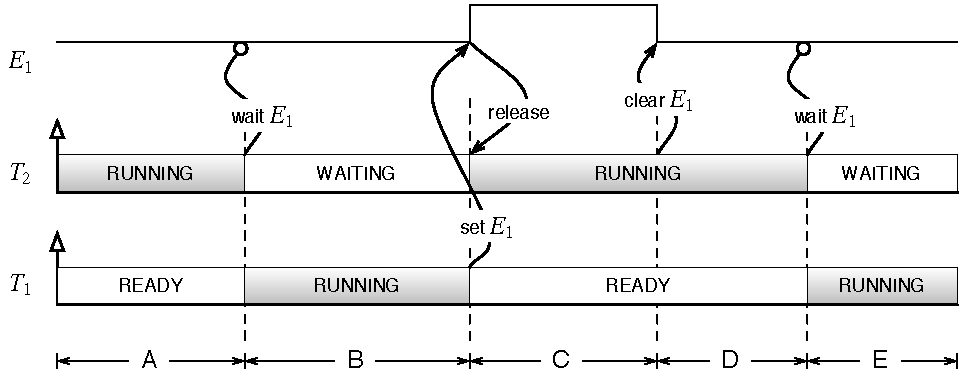
\includegraphics[scale=.7]{pictures/schedulingEvent.pdf} 
   \caption{{\bfseries Scheduling with an event.}  $T_2$ is an extended task. During A period, $T_2$ is {\sffamily\scshape running} and $T_1$ is {\sffamily\scshape ready}. Then $T_2$ wait for $E_1$ and blocks. $T_2$ runs (B period) and sets $E_1$. $T_2$ is released and since $P(T_2)>P(T_1)$, $T_2$ runs (C period), clears $E_1$ and continues to run (D period). Then $T_2$ wait for $E_1$ again and blocks, $T_1$ runs (E period).}
   \label{fig:scheduleEvent}
\end{figure} 


\warning{Events must be explicitly cleared once read. If a tasks does not clear the previous occurrence of an event, it will be seen as ``already occurred'' the next time the task will wait for it.}
 

\section{OIL description}

An event is described using a \oilattr{EVENT} object. \oilattr{MASK} is the single attribute of this object. \oilattr{MASK} may be set to a literal value:

\begin{lstlisting}[language=OIL]
EVENT ev {
  MASK = 0x1;
};
\end{lstlisting}

\note{The literal value should have  only 1 bit set. Goil emits a warning when this is not the case.} 

Or \oilattr{MASK} may be set to \oilattr{AUTO}. In this case, the \sysgen\ computes the event mask:

\begin{lstlisting}[language=OIL]
EVENT ev {
  MASK = AUTO;
};
\end{lstlisting}


\section{Events services}

\begin{service}{SetEvent}{StatusType}
Events of task \var{TaskID} are set according to the Mask passed as $2^{nd}$ argument. This service is non blocking and may be called from a task or an ISR2.

\note{\servicename\ may do a rescheduling if the target task is unblocked and goes to the \READY\ state.}

\argument{TaskType}{TaskID}{the id of the task}
\argument{EventMaskType}{Mask}{the event mask}
\resultcode{\OK}{No error}
\resultcodeext{\OSID}{Invalid TaskID}
\resultcodeext{\OSACCESS}{TaskID is not an extended task (not able to manage events)}
\resultcodeext{\OSSTATE}{Events cannot be set because the target task is in the \SUSPENDED\ state}
\end{service}


\begin{service}{WaitEvent}{StatusType}
The calling task waits for event(s) \var{Mask}. If one the events are already set, the task continues its execution. If none of the events are set, the task is put in the \WAITING\ state and blocks.

\note{\servicename\ may do a rescheduling if the calling task blocks.}

\argument{EventMaskType}{Mask}{The event(s) to wait for}
\resultcode{\OK}{No error}
\resultcodeext{\OSACCESS}{The calling task  is not an extended task (not able to manage events)}
\resultcodeext{\OSRESOURCE}{The calling task holds a resource}
\resultcodeext{\OSCALLLEVEL}{The caller is not a task}

\end{service}

\begin{service}{GetEvent}{StatusType}
Events of task \var{TaskID} are copied in \var{Mask} argument passed as reference.

\note{\servicename\ does not reset the event mask. \api{ClearEvent} should be used to clear, in the event mask, the events that have been processed.}

\warning{The \var{Mask} argument is a pointer. Do not pass an uninitialized pointer. Proper use of this service supposes a \ctype{EventMask} variable is instantiated, then its address is passed to \cfunction{\servicename} as shown in the example below:}

\begin{lstlisting}[language=C]
EventMaskType myEventMask;
GetEvent(aTask, &myEventMask);
\end{lstlisting}

\argument{TaskType}{TaskID}{the id of the task}
\argument{EventMaskRefType}{Mask}{the reference of the event mask where the \var{TaskID} event mask is copied}
\resultcode{\OK}{No error}
\resultcodeext{\OSID}{Invalid TaskID}
\resultcodeext{\OSACCESS}{The task identified by TaskID is not an extended task (not able to manage events) or, in \autosar, the caller cannot access the task}
\resultcodeext{\OSSTATE}{The task identified by TaskID is in \SUSPENDED\ state}
\end{service}